%!TEX root = ../icip_jseo.tex
% -*- root: ../icip_jseo.tex -*-


\section{Related Works}
\label{sec:relworks}

%하지만 이러한 feature matching 기반의 markerless AR 알고리즘은 연산량이 많기 때문에 mobile phone과 같은 smart space 환경에서는 자연스러운 동작이 어렵다. 이를 극복하기 위하여 다양한 경량화 알고리즘들이 제안되고 있다. 특히, 그림 xxx\todo{매칭 속도 비교 새 버전 입력}에서 보듯이 전체적인 연산 성능에 큰 영향을 미치는 단계인 feature description과 matching 단계에 대한 속도 향상이 많이 이루어지고 있다.



%먼저, keypoint descriptor는 기존의 SIFT\cite{lowe_distinctive_2004}나 SURF\cite{bay_speeded-up_2008}와 같은 vector value-based description 방법은 높은 인식율을 제공해 주었지만, orientation과 scale 등의 distortion에 robust한 descriptor를 생성하기 위하여 복잡한 연산을 수행하여야 하기 때문에 연산이 복잡하게 수행되었다. 따라서 최근에는 BRIEF\cite{calonder_brief:_2010}, ORB\cite{rublee_orb:_2011}, BRISK\cite{leutenegger_brisk:_2011}, FREAK\cite{alahi_freak:_2012}과 같은 다양한 Binary value-based descriptor들이 개발되고 있다. 이러한 Binary descriptor들은 그림 xxx\todo{binary desciprot 패치 }와 같이 특징점을 중심으로 다양한 형태의 패턴을 이용하여 두 점 사이의 밝기 값을 비교하여 binary code로 표현하는 방법이다. 단순 비교 연산만으로 descriptor를 계산하기 때문에 vector-based descriptor에 비하여 연산 속도가 상당히 빠르며, 최근에는 생성 패턴을 기준으로 orientation이나 scale 등을 normalize 하기 때문에 다양한 distortion에서도 상당히 강인한 성능을 보여주고 있다. 특히 smart space와 같이 제한된 성능의 환경에서는 vector-value descriptor 기반의 복잡한 연산 보다는 단순 비교연산만으로도 처리가 가능한 binary descriptor를 사용하는 연구가 많아지고 있다. 

In spite of robust matching quality, keypoint-based local matching requires a large amount of computation, especially in mobile computing environment. To overcome this limitation, various lightweight algorithms are proposed. At first, in the study of keypoint descriptors, the vector-value based description methods such as SIFT\cite{lowe_distinctive_2004} or SURF\cite{bay_speeded-up_2008} provide robust recognition quality, but complex computation is required to calculate descriptors. In recent years, variant binary-value based descriptors, such as  BRIEF\cite{calonder_brief:_2010}, ORB\cite{rublee_orb:_2011}, BRISK\cite{leutenegger_brisk:_2011}, FREAK\cite{alahi_freak:_2012}, are proposed. These binary descriptors compare the brightness values with focus on the keypoints as shown in Figure \ref{fig:markerless_binary_patterns} by using a wide range of form patterns and express the results in binary codes. Since descriptors are computed only by a simple comparison computation, its computational speed is significantly faster than vector-based descriptors. Moreover, since the orientation and scale are normalized on the basis of generation patterns, they show significantly robust performance against a wide range of distortion. In particular, studies using the binary descriptors that can be processed by simple comparison computation rather than complex vector-value descriptor based computation are increasing in the environment of limited performance such as a mobile computing.  

\begin{figure}[hb!]
  \centering     %%% not \center
    \subfigure[BRISK\cite{leutenegger_brisk:_2011} Sampling Pattern]{\label{fig:markerless_brisk}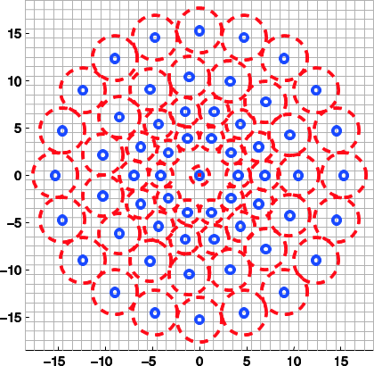
\includegraphics[width=0.48\columnwidth]{2_relworks/brisk}}
    \hfill
    \subfigure[FREAK\cite{alahi_freak:_2012} Sampling Pattern]{\label{fig:markerless_freak}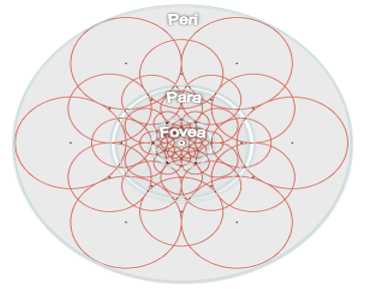
\includegraphics[width=0.48\columnwidth]{2_relworks/freak}}
  \caption{Sampling Patterns of Binary Descriptors}
    \label{fig:markerless_binary_patterns}
\end{figure}


%다음 방법은 matching data structure를 효율적으로 설계하여 nearest neighbor match를 빠르게 수행하도록 하고 있다. 기존의 brute force matching 방법은 query image의 모든 keypoint들을  reference image의 모든 keypoint들과 비교하는 방식으로 가장 속도가 오래 걸리지만, 가장 정확한 nearest neighbor를 검출할 수 있다는 장점이 있다. 이를 개선하기 위하여 다양한 tree 기반의 approximated nearest neighbor 검출 기법들이 사용된다. \cite{beis_shape_1997}에서는 kD tree 기반의 approximation 방법이 제안되었다. 이 방법은 특징의 차원이 비교적 적은 SIFT나 SURF와 같은  vector-value description 방식에서는 좋은 성능을 보여주지만, 최근에 사용되는 binary descriptor에서는 dimension이 높아 성능향상을 기대하기 어렵다는 문제가 있다. LSH\cite{gionis_similarity_1999}와 같은 Hashing 기반의 structure를 이용하여 matching 을 가속화하는 방법도 제안되었다\cite{rublee_orb:_2011}. 이러한 방법은 offline training 단계에서 적절히 특징점들이 고르게 분포하도록 적절한 hash function set을 구성하는 것이 중요하다. 또한, Random Forest\cite{lepetit_keypoint_2006} 또는 Random Fern \cite{ozuysal_fast_2010}은 Binary Description 방식을 Tree 구조 또는 List 구조에 적용하여 matching structure를 구성하였다. 이러한 매칭 방식들은 인식의 속도를 향상시키고, 좀 더 정확한 approximation 값을 얻기 위하여 일반적으로 offline training 단계에서 계산된 descriptor들을 이용하여 추가의 연산을 적용하여 효율적인 matching structure를 생성한다. 하지만, 이러한 방법들을 사용한 추가적인 구조체가 상당히 복잡하고 용량이 크기 때문에 모바일 환경에서 사용하기에 매칭 구조체가 과도하게 무거워진다는 문제점이 존재한다. 또한, detected keypoint의 성질에 대한 고려가 없기 때문에 detected keypoint set이 분류가 어려운 set 일 경우에는 성능 저하가 크게 된다는 한계가 존재한다. 따라서 본 학위논문에서는 이러한 방법을 해결하기 위하여 Keypoint Filtering 기반의 향상된 매칭 방법을 제안한다.

The other researches accelerates nearest neighbor matching with designing an efficient matching data structure. The conventional brute force matching compares all the keypoints of query images with all the keypoints of reference images, so it shows the slowest, but has the advantage of being able to detect the most accurate nearest neighbors. kD tree based approximation method is proposed in \cite{beis_shape_1997}. This method shows good performance in the vector-value descriptor method such as SIFT or SURF with relatively low dimension of features but the improvement of its performance is unlikely to be achieved in the latest binary descriptor with high dimension. A method enabling it to accelerate matching using Hashing based structure in LSH\cite{gionis_similarity_1999} was proposed\cite{rublee_orb:_2011}. As for this method, it is critical to compose appropriate hash function set to distribute the keypoints points evenly in the offline training phase. In addition, 'Random Forest\cite{lepetit_keypoint_2006}' or 'Random Fern\cite{ozuysal_fast_2010}' composed a matching structure by applying a binary description method to the tree structure or list structure. To increase the recognition speed and obtain more accurate approximation values, these matching methods generate efficient matching structure by way of the application of supplementary computation using the descriptors computed in the offline training phase. However, since the supplementary structure that uses this method is complex and large, its the matching structure is too heavy to use in a mobile environment. Moreover, since the properties of the detected keypoints are not taken into consideration, the set for which it is difficult to classify the detected keypoints may lead to performance degradation. To solve this problem, this dissertation proposes a keypoints filtering based matching methods.  
